\chapter{Implementing the Spacetime}
\label{chap:implementing-gr}

In the QFT implementation chapter, we briefly touched on GR, since space and time are the necessary background that QFT needs to define its fields.
In truth, downplaying GR as 'no big deal' wasn't entirely fair.

Anyone familiar with GR most likely laughed while reading that—or perhaps cried, or more likely both.

To get any sense out of GR, let's implement it.


\section{The Spacetime Implementation}

In a rigorous object-oriented implementation of General Relativity, one does not store forces or arbitrary gravitational fields. 
The universe is modeled as a structural interplay between an abstract base \textbf{Tensor} data container and its specialized geometric and energy variants.

Crucially, because we inhabit a static Block Universe, the components of these tensors are not stored as static, dead scalar primitives like floating-point arrays. 
Instead, every component is a continuous \textbf{ScalarField}---a functional object that takes an explicit four-dimensional coordinate position $(t, x, y, z)$ and evaluates the local mathematical value on the fly.

\begin{lstlisting}[language=C++, caption=The Core Tensor Architecture]

#include <functional>
#include <array>
#include <cmath>

/**
 * Represents a single event or point in the 4D spacetime manifold.
 */
struct Position4 {
  double t, x, y, z;
};

using ScalarField = function<double(const Position4& pos)>;

/**
 * Abstract base class representing a Rank-2 Spacetime Tensor.
 */
class Tensor {
  array<array<ScalarField, 4>, 4> components;
  virtual ~Tensor() = default;
  
  ScalarField getComponent(int mu, int nu) const { 
    return components[mu][nu]; 
  }
};

/**
 * The Metric Tensor (g_mu_nu).
 */
class MetricTensor : public Tensor {
  Tensor getInverse() const; // Contravariant metric (g^mu_nu) 
  Tensor getEinsteinTensor() const;
  
  array<array<array<ScalarField, 4>, 4>, 4> getChristoffel() const;

  /**
   * Evaluates a geodesic worldline step at a specific coordinate location.
   * The trajectory is determined by evaluation of the Christoffel fields.
   */
  array<double, 4> computeGeodesicAcceleration(const Position4& pos, 
                                                array<double, 4> velocity) const {
    array<double, 4> acceleration = {0.0, 0.0, 0.0, 0.0};
    auto Gamma = this->getChristoffel();
    
    for (int mu = 0; mu < 4; mu++) {
      for (int nu = 0; nu < 4; nu++) {
        for (int rho = 0; rho < 4; rho++) {
          // Evaluate the field at this specific event
          double gamma_val = Gamma[mu][nu][rho](pos);
          acceleration[mu] -= gamma_val * velocity[nu] * velocity[rho];
        }
      }
    }
    return acceleration; 
  }
};

class StressEnergyTensor : public Tensor {};

/**
 * The universe, cosisting of energy and spacetime geometry
 */
class Universe {
  const double G = 6.6743e-11;
  const double c = 299792458.0;

  MetricTensor g_mu_nu;
  StressEnergyTensor T_mu_nu;

  /**
   * Assert the field equations locally at a specific spacetime event.
   * G_mu_nu == (8 * pi * G / c^4) * T_mu_nu
   */
  bool EFE(const Position4& pos) const {
    auto G_tensor = g_mu_nu.getEinsteinTensor();
    double constant = (8.0 * M_PI * G) / pow(c, 4);

    for (int mu = 0; mu < 4; mu++) {
      for (int nu = 0; nu < 4; nu++) {
        double geometry_val = G_tensor.getComponent(mu, nu)(pos);
        double energy_val = T_mu_nu.getComponent(mu, nu)(pos);
        
        if (abs(geometry_val - (constant * energy_val)) > 1e-9) {
          return false; 
        }
      }
    }
    return true;
  }
};

\end{lstlisting}

The complexity of GR emerges from the fact that the system writes back to itself. 

The matter-energy values of QFT (the \textbf{Stress-Energy Tensor}, $T_{\mu\nu}$) specify the functional constraints of the Metric ($g_{\mu\nu}$).
Because the geometry of the metric changes how fields evaluate across coordinates, it alters the path of the stress-energy distribution. 
This creates a highly non-linear, self-referential loop. 
In software terms, it is a recursive function where the stack frame itself is constantly warping while the function executes.


\subsection*{The Class Diagram}

To sum it up, spacetime is the interplay of exactly two components: 

\textit{Energy} ($T_{\mu\nu}$): The physical content—mass, radiation, pressure, and momentum.

\textit{Geometry} ($g_{\mu\nu}$): The measurement framework—distances, time intervals, curvature, and causal pathways.

Einstein’s field equation is the equal sign between them. 

\begin{figure}[h]
\centering
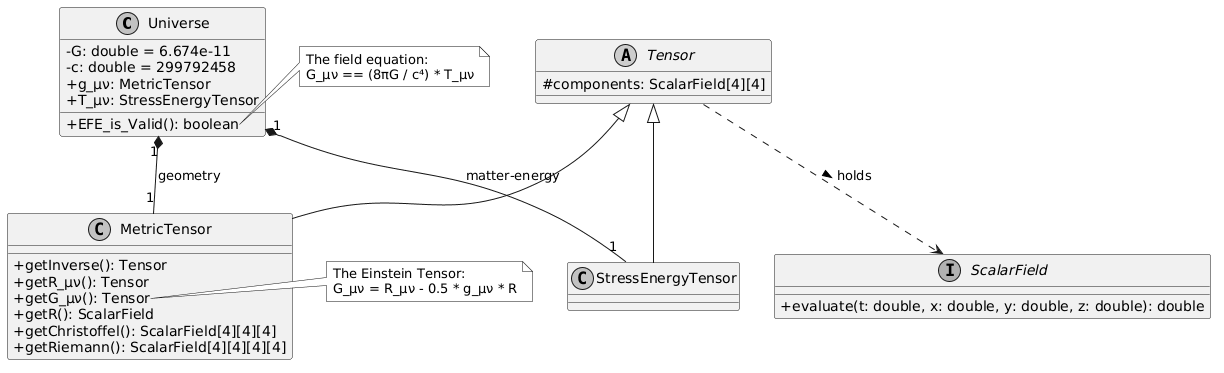
\includegraphics[width=1.0\textwidth]{figures/gr-class-diagram.png}
\caption{\emph{General Relativity UML Diagram}}
\end{figure}


\section{Minor Implementation Notes}

Awesome. we'll just write a quick Runge-Kutta integrator, set up a 4D grid, write a finite-difference stencil for the Einstein Field Equations, and simulate a binary black hole merger by next weekend.

While the core equation of GR ($G_{\mu\nu} = \frac{8\pi G}{c^4} T_{\mu\nu}$) looks deceptively simple, expanding it yields a system of ten coupled, highly non-linear, hyperbolic-elliptic partial differential equations.

If one tries to write a naive solver, the simulation will face-plant into several classic software-engineering traps, such as coordinate singularities.
Simulation will crash with a \texttt{NaN} or overflow error. Resolving these requires advanced mathematical coordinate transformations (like Kruskal-Szekeres coordinates or "moving puncture" gauge conditions) just to keep the grid mathematically stable.

Constraint Violations emerge because the Einstein equations are split into "evolution equations" (which update the grid over time) and "constraint equations" (which must remain true at every single step, like $\text{div}(B) = 0$ in electromagnetism).
In a naive simulation, numerical rounding errors will accumulate.  Within a few frames, the constraint equations will fail, meaning the spacetime grid no longer has any physical meaning.

To resolve the high-frequency gravitational waves radiating from a binary merger one needs Adaptive Mesh Refinement (AMR).
Writing a dynamically scaling, parallelized 4D grid that runs efficiently across thousands of GPU nodes is a multi-decade software engineering challenge.

Fortunately, the open-source community has already built the frameworks so we don't have to. We can use the industry-standard, production-ready engines:
\begin{itemize}
\item \textbf{The Einstein Toolkit:} The Kubernetes of numerical relativity.
  It is a massive, community-driven, high-performance computing framework built on the Cactus infrastructure.
  It handles everything from the 3+1 spacetime decomposition to adaptive mesh refinement and relativistic hydrodynamics.
\item \textbf{NRPy+ (Python-based Code Generation):} A brilliant Python package that uses SymPy to let you write your physics equations in clean, high-level Einstein notation.
  It then compiles those equations into highly optimized, SIMD-parallelized C++ code.
  It is designed to lower the barrier to entry, letting you run numerical relativity on a standard laptop.
\item \textbf{OGRePy / xAct / SageManifolds:} If you don't need a full-blown dynamic simulation and just want to do symbolic tensor algebra (e.g., calculating Christoffel symbols, Riemann curvature, or geodesics from a given metric), do not do the derivatives by hand.
\end{itemize}



\section{Conclusion}


Let's compare this to our implementation of Quantum Field Theory. 

In the grand hierarchy of the universal source code, it is clear that while the Standard Model was written by a committee of panicked, underpaid junior developers working on a Friday afternoon, General Relativity was designed by a single Senior Architect during a moment of pure, uninterrupted clarity.

Compared to the cluttered, variable-heavy spaghetti code of QFT—with its arbitrary coupling constants,
messy exclusion rules, and infinite loops that require "renormalization" hacks just to keep the compiler from crashing—General Relativity is architecturally superior in every way. 

The architect responsible for this module surely deserves a raise.

